\section{Approach}
\label{sec:approach}

This work describes {\it Pythia},\footnote{Pythia
will be available as open source code.
Locations not shown for double-blind reviewing}
an approach that analyzes applications,
to identify data-paths
which involve dangerous constructs such
as the ones described in Section~\ref{sec:motivation}.
To do so,
Pythia analyzes an application's
views and templates,
leaving out models as they do not hold any relevant information.
Figure~\ref{fig:arch} presents the basic steps performed by our approach:
First,
Pythia searches for specific constructs,
which we call {\it sinks},
marking any affected templates and then,
examines views to identify
\textbf{(1)} if untrusted data can reach
the elements identified in the first step,
\textbf{(2)} if other sinks are being used by the views.

\begin{figure}[t]
    \begin{center}
        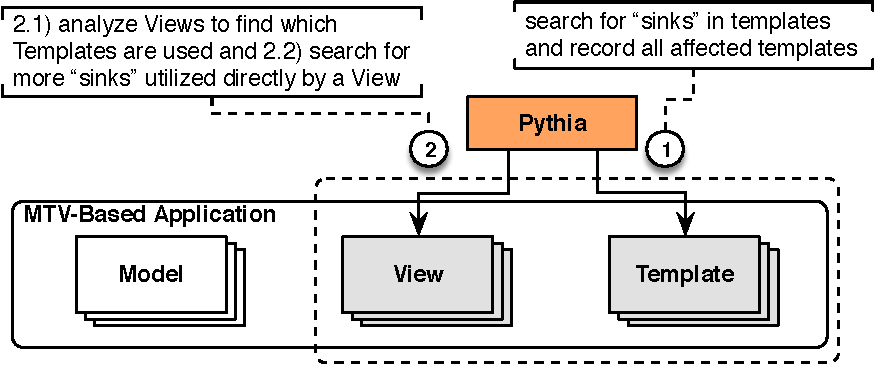
\includegraphics[scale=0.53]{MVC_and_Pythia_2.pdf}
        % \vspace{-2mm}
        \caption{In the Model Template View ({\sc mtv}) Context, {\it Pythia} focuses on {\tt Views} and {\tt Templates}.}\label{fig:arch}
    \end{center}
    % \vspace{-3mm}
\end{figure}

\subsection{Sinks}
\label{sec:sinks}

A sink method depicts a coding construct
where the hazard might take place~\cite{MLPK17}.
In our case,
a sink involves an invocation that bypasses
the default security mechanisms of a Django
Application.
In such an application we can divide sinks
into two categories,
namely:
{\it in-view sinks},
and {\it template sinks}.
The first category
only affects a particular {\tt View},
while the second on involves templates
that may affect all the views that use them. 

{\it Template Sinks} involve Django filters
such as {\tt safe} and {\tt safeseq},
and tags such as {\tt autoescape}.
The {\tt autoescape} tag,
controls the auto-escaping effect of a code block.
When disabled (set to {\tt off}),
it is equivalent to marking all variables
inside that code block as ``safe".
Escaping concerns dangerous characters
such as '{\tt <}', which in turn is 
converted to '{\tt \&lt;}' and more.
Furthermore,
filters including {\tt safeseq} and
{\tt safe} dictate that a variable
does not require further {\sc html} escaping
before it becomes part of  the output.

{\it In-view Sinks} include {\it decorators}
such as {\tt @csrf\_exempt} and functions
invocations that can lead to {\sc xss}
defects when used in an improper manner
(e.g. {\tt mark\_safe}).

To trace dangerous data flows,
Pythia expects as input two lists which in turn
include the constructs of each category.
The lists, can easily be expanded with more methods 
depending on the needs of the developer,
thus providing flexibility to track other 
application / project-specific filters
or decorators.

When Pythia identifies a sink,
it then examines the application
for potential sources,
i.e. variables that hold data that
can reach the sink.
Notably,
such data can come from a {\tt Model}
or a user request
(e.g. {\tt request.GET.get()}).
In the upcoming section we discuss
how Pythia examines the various data paths
of an application.

\begin{algorithm}[t]
\caption{Searching for Dangerous Flows}
\label{alg:explore}
\begin{algorithmic}[1]
\State {\bf INPUT} $TS$: template sinks
\State {\bf INPUT} $IS$: in-view sinks
\State {\bf INPUT} $url\_conf$: the {\tt urlpatterns} object containg all URLs
\Function{analyze}{$TS$, $IS$, $url\_conf$}
\State $S \gets set();$

\State $T \gets getTemplates();$
\Comment{ Stage 1 }
\State $paths[];$

\ForAll{$t \in T$}
    \State $t.walk(TS, paths[], t.root, t.name);$
\EndFor
\State $V \gets getAllViews(url\_conf);$
\Comment{ Stage 2 }
\ForAll{$v \in V$} 
    \If{$v.invokes(IS)$}
        \State $S.add(v);$
    \EndIf
    \ForAll{$p \in paths[]$}
        \If{$v.renders(p)$}
            \State $S.add(v, p);$
        \EndIf
    \EndFor 
\EndFor
\EndFunction
\end{algorithmic}
\end{algorithm}

\subsection{Application Analysis}
\label{sec:analysis}

Algorithms~\ref{alg:explore}
and~\ref{alg:paths} illustrate
how Pythia examines a Django application.
First,
our approach retrieves all project templates
and generates their corresponding
Abstract Syntax Trees ({\sc ast}s).
Then,
starting from the root node of each {\sc ast},
it recursively traverses all children
nodes searching for variables that
reach a sink method.
This process starts in line 9
of Alg.~\ref{alg:explore} and continues
in Alg.~\ref{alg:paths}.
Specifically,
when Pythia identifies a sink,
it marks the template as potentially
dangerous (Alg.~\ref{alg:paths}, line 9).
If the current template extends or
includes another one,
the approach goes on to examine
the other template too
(Alg.~\ref{alg:paths}, lines 10-13).
In this way it creates a path that
is recorded when a sink is found.
When a potentially dangerous path is found, the current node 
and the template ancestry are kept in a key-value store in 
order to be cross-examined in the second stage.

When the first part finishes,
Pythia analyzes the views of the application
and extracts all decorators.
Then,
it traverses the {\sc ast} of each {\tt View}
to identify the templates that are being used
and the data that each template requires 
to render the page.
Finally,
the results are 
being cross-examined in order to find
unsafe data paths.

\begin{algorithm}[ht]
\caption{Exploring Paths}
\label{alg:paths}
\begin{algorithmic}[1]
\State {\bf INPUT} $TS$: template sinks
\State {\bf INPUT} $paths[]$: a list holding all
potentially tainted paths
\State {\bf INPUT} $node$: current {\sc ast} node
\State {\bf INPUT} $origin$: template ancestry
\Function{walk}{$TS$, $paths[]$, $node$, $origin$}
\ForAll{$subnode \in node.nodelist$}
    \If{$subnode.isVariable()$}
        \If{$subnode.invokes(TS)$}
            \State $paths[] \gets subnode, origin;$
        \EndIf
    \ElsIf{$subnode.isExtendsNode()$}
        \State{$walk(TS, paths, subnode, subnode.extended\_template)$}
    \ElsIf{$subnode.isIncludeNode()$}
        \State{$walk(TS, paths, subnode, subnode.included\_template)$}
\EndIf
\EndFor
\EndFunction
\end{algorithmic}
\end{algorithm}

\subsection{Resolution of Paths}
\label{sec:output}

The output of Pythia is based on the
category of the sink identified.
In the case of a decorator
(i.e an in-view sink such as
{\tt \@csrf\_exempt}),
the output contains:
(1) the {\sc url} under
which the potentially vulnerable
view resides,
(2) the module where the view is defined
(the last component of the module is the view's name), 
and (3) which decorators were used on it.

If a dangerous function is identified within a view,
Pythia returns (1) the view's corresponding
{\sc url} (e.g. /users/<id>/),
(2) the module where the view is defined
alongside with the line under where
the function was invoked,
(3) the function's name,
and (4) the variable it was ran upon.

For template sinks,
Pythia's output includes all views that render,
directly or indirectly,
a template that uses the list of
unsafe filters and tags.
In addition,
it contains the module and the line where
the view is defined,
the ancestry path to reach the dangerous template,
the filter that was applied,
the variable itself,
and the variable's context.
\footnote{The term context is used to describe all variable aliasing / assignments
within the current scope, until a dangerous filter invocation is reached.}
Note that the context information is needed
to track the data provided from the view to
the template until they reach the sink.

Furthermore,
in case a specific template containing sinks
does not resolve to a view,
the path to the sinks is still part of the output.
In this manner,
a security expert can manually resolve
the given template until the source
of the data is found.
An example where the full path is not
resolved is when a template is used
for the rendering of a form inside a template.
Currently,
Pythia does not go through form definitions
to find template invocations.

\subsection{Output Filtering}
\label{sec:filtering}

As we discussed earlier Pythia
outputs a number of potentially
dangerous data paths.
This means that a part of a path
may appear in other several paths.
In addition,
a template that marks output
as safe may be included by multiple
templates.
In such occasions the output of
the tool may include recurring information
with duplicated elements.

To reduce the volume of such instances
we apply filters that make the output
more comprehensive and easy to use.
For instance,
we enumerate the views that end up
using a template including {\tt safe} tags
and let the user explore their names as a
second step.

\subsection{Implementation Details}
\label{sec:implementation}

In the scope of Django applications that 
Pythia analyzes, this section provides 
a number of details regarding
the tool's implementation and its internals.

As mentioned earlier, Pythia requires the {\sc ast} of a
template. To generate the {\sc ast} of a template,
Django requires a running environment.
This is because Django needs to resolve
user-defined components (e.g. custom filters)
and its own defaults (e.g. for loops, variable aliasing).
Other operations such as the analysis of a view's
module are realized statically using Python's
{\sc ast} package.

This design decision, to divide the implementation
between purely static and processes that require
Django's run-time to be setup has certain
assets and liabilities.
Using a purely static approach,
one can easily use the tool on many projects
without having to configure their dependencies
and requirements,
and even run it during a project's continuous
integration as another security test.
However,
with the hybrid approach one can gain the
advantage of having the ability to use
certain aspects of Python's and Django's
run-time and exploring paths that
otherwise would not be possible to explore. 

Regarding further implementation details, 
Pythia supports both Python 2.x and 3.x
versions and Django 1.8.x until 1.11.x. Versions 
before 1.7.x, are not supported as they have a
vastly different internal representation
of the {\sc ast} node classes.
